\section{Introduction}
This article synthesizes three crucial aspects: the opportunities and associated risks of AI technologies in fostering human dignity and promoting flourishing, the principles underlying AI adoption, and specific recommendations for stakeholders to seize opportunities, mitigate risks, respect principles, and develop a Good AI Society.

\section{The Opportunities and Risks of AI for Society}

\subsection{Who We Can Become: Enabling Human Self-Realization}
AI holds the potential to allow individuals to spend their lives more intelligently, facilitating personal growth and self-improvement. However, the rapid pace of change might cause challenges as jobs and skills evolve. Fostering AI in support of new skills while mitigating its impact on traditional ones requires close study and innovative ideas like a "universal basic income" to ensure a fair transition to the future.

\subsection{What We Can Do}
AI offers a reservoir of "smart agency," augmenting human capabilities. Responsibility in deploying AI is crucial to prevent the absence of accountability. The relationship between human agency and autonomous systems isn't necessarily contradictory. Thoughtful development of AI can expand human possibilities and should focus on enhancing human potential rather than diminishing it.

\subsection{What We Can Achieve}
AI-augmented human intelligence presents solutions to old and new problems, from resource distribution to sustainable consumption. However, over-reliance on AI might lead to delegating important decisions to autonomous systems. Striking a balance between leveraging AI opportunities and retaining control over major developments is imperative.

\subsection{How We Can Interact}
Global challenges demand collaboration among stakeholders. AI can address coordination complexity, such as tackling climate change. Radical choices like societal restructuring or "self-nudging" through AI raise concerns about unintentional changes in human behavior that could erode self-determination. Designing AI systems to encourage positive behavior while respecting autonomy is crucial.

\begin{figure}[h]
    \centering
    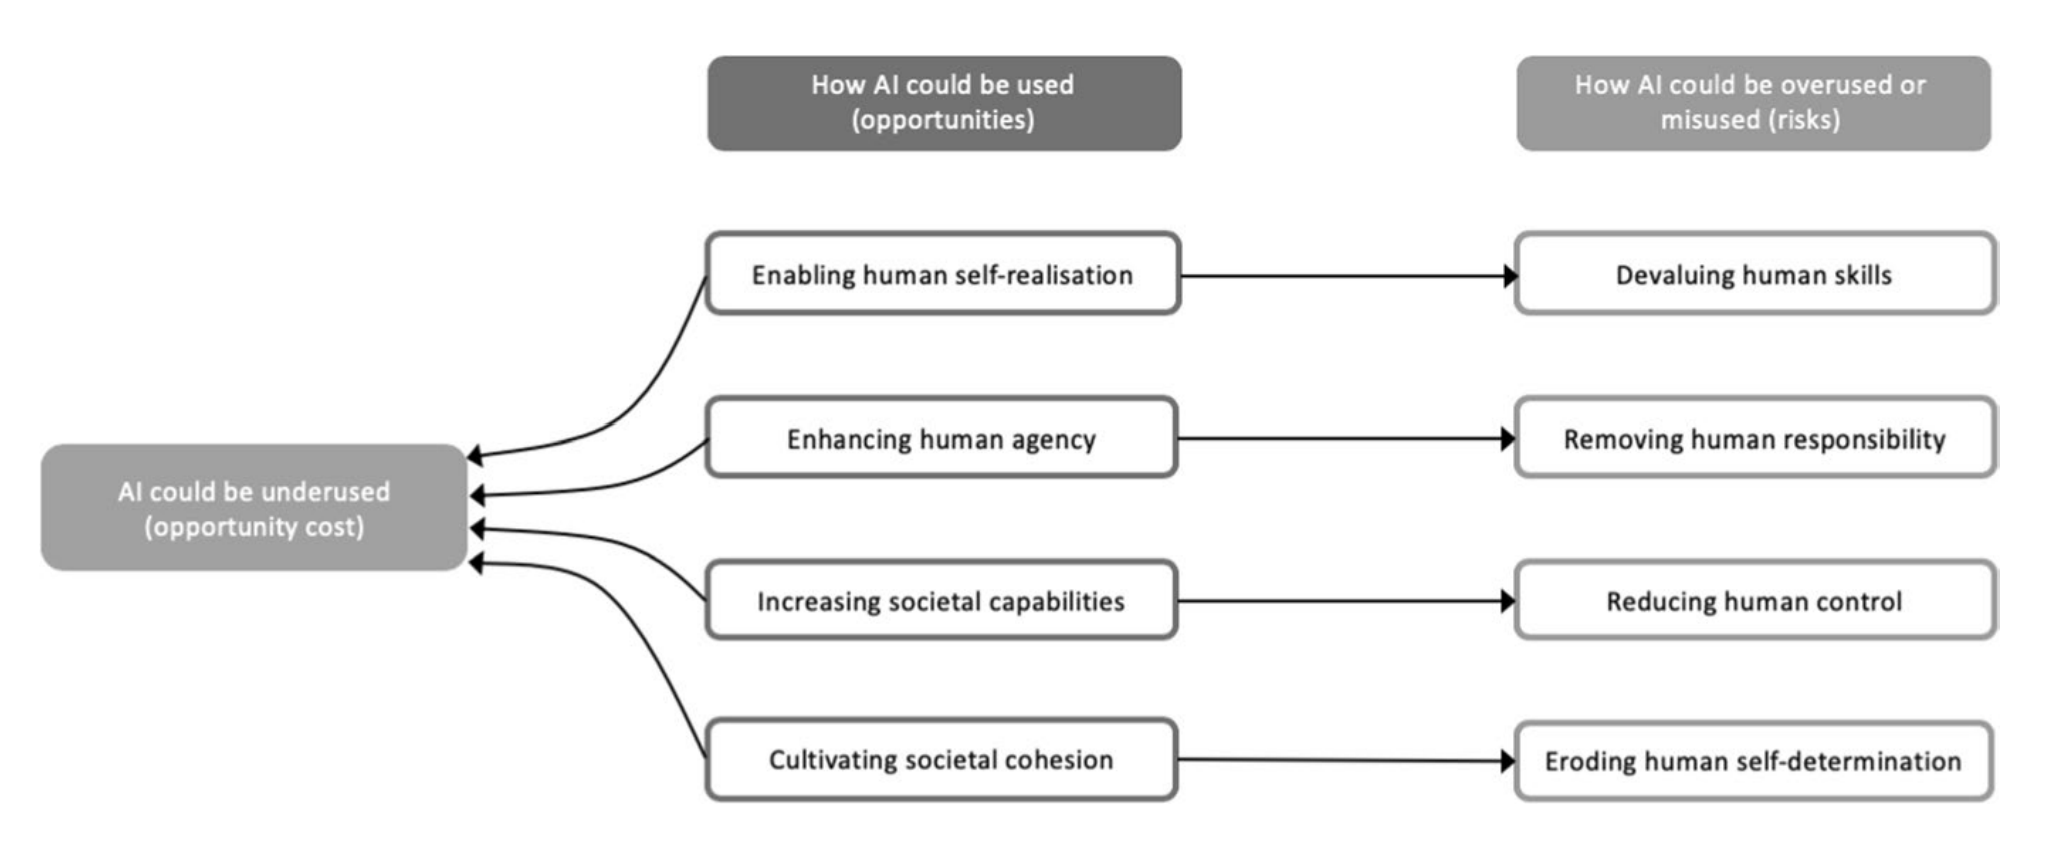
\includegraphics[width=0.75\linewidth]{Assets/AI Overview.png}
    \caption{Overview of the four core opportunities offered by AI, four corresponding risks, and the opportunity cost of under-using AI}
    \label{fig:Ai-overview}
\end{figure}

\section{Foundational AI Adoption Principles}

\subsection{The Dual Advantage of an Ethical Approach to AI}
Achieving socially preferable outcomes through AI involves reconciling the benefits while mitigating potential harms. Compliance with the law is necessary but insufficient; it's akin to playing by the rules rather than excelling to win the game. Adopting an ethical approach to AI offers what we term a "dual advantage."
Ethics in AI confers this dual advantage. Firstly, it empowers organizations to capitalize on the social value that AI can bring. This advantage lies in identifying and leveraging opportunities that align with societal values. Secondly, ethics aids in anticipating, avoiding, or minimizing costly mistakes. It acts as a preventative measure, mitigating actions that might be legally sound but socially unacceptable. This approach reduces the opportunity costs associated with choices made out of fear of potential mistakes.
For ethics to wield its dual advantage, it necessitates an environment of public trust and clear responsibilities. These attitudes hinge on public engagement with AI technology development. 

\subsection{Framework of Principles}
AI4People isn't the pioneer in considering the ethical implications of AI; there are six other documents addressing this. 
\begin{enumerate}
    \item The Asilomar AI Principles (2017)
    \item The Montreal Declaration for Responsible AI (2017)
    \item The General Principles offered in the second version of Ethically Aligned Design (2017)
    \item The Ethical Principles offered in the Statement on Artificial Intelligence, Robotics and ‘Autonomous’ Systems (2018)
    \item The “five overarching principles for an AI code” (2018)
    \item The Tenets of the Partnership on AI (2018)
\end{enumerate}

Together, these documents present 47 principles.

\paragraph{Beneficence: Promoting Well-being, Preserving Dignity, and Sustaining the Planet}
Among the core bioethics principles, beneficence is notably prominent across the six synthesized sets of principles. The commitment to creating AI technology that benefits humanity is a consistent priority across these principles.

\paragraph{Non-maleficence: Privacy, Security, and "Capability Caution"}
While "do only good" (beneficence) and "do no harm" (non-maleficence) might seem logically similar, they represent distinct principles in both bioethics and AI ethics. Privacy infringements stand as a primary concern, yet it's not the sole peril; other misuses of AI technology are highlighted. The Asilomar Principles specifically address the threats of an AI arms race and recursive self-improvement, emphasizing "caution" regarding "upper limits on future AI capabilities." Clarity is lacking on whether it's the developers or the technology itself that should avoid harm. Intent, whether accidental ("overuse") or deliberate ("misuse"), is incorporated into the concept of promoting non-maleficence.

\paragraph{Autonomy: The Power to Decide (Whether to Decide)}
An essential bioethics principle, autonomy asserts individuals' right to decide on their treatment. This principle extends beyond human autonomy; it encompasses regulating machine autonomy, making it intrinsically reversible if human intervention becomes necessary (e.g., a pilot turning off automatic pilot to regain control). Protecting human choice's intrinsic value, particularly in significant decisions, aims to limit excessive delegation to machines. Any delegation should remain overridable in principle, allowing the choice to decide again.

\paragraph{Justice: Promoting Prosperity and Preserving Solidarity}
Justice, a classic bioethics principle, pertains to resource distribution, including access to experimental treatments or general healthcare availability. In the context of AI, it emphasizes the need for "shared benefit" and "shared prosperity" and warns against biases in AI training datasets. It raises questions about whether humans are the patient receiving AI's "treatment," the prescribing doctor, or both.

\paragraph{Explicability: Enabling the Other Principles Through Intelligibility and Accountability}
Addressing the question of whether "we" are the patient or the doctor depends on circumstances and perspectives. The unequal involvement of a fraction of humanity in AI technology design and its transformational impact on everyone else necessitates understanding and holding AI decision-making processes accountable. Explicability, synthesized as "intelligibility" and "accountability," fills a crucial gap in applying bioethics to AI ethics. \newline

Collectively, these five principles encapsulate the essence of the 47 principles from the six documents, forming an ethical framework.

\begin{itemize}
    \item \textbf{Assessment}
    \begin{enumerate}[label*=\arabic*.]
        \item \textbf{Assess institutional capacity} to address AI-related mistakes or harms, considering liability from design to reduce negligence.
        \item \textbf{Evaluate which tasks shouldn't be delegated} to AI, aligning with societal values and public opinion.
        \item \textbf{Review regulations' ethical grounding} for a flexible legislative framework, including principles for urgent issues.
    \end{enumerate}

    \item \textbf{Development}
    \begin{enumerate}[label*=\arabic*.]
        \setcounter{enumi}{3}
        \item \textbf{Enhance explicability} of socially impactful AI systems, providing clear explanations in case of unintended consequences.
        \item \textbf{Improve legal procedures} for scrutinizing algorithmic decisions in court, considering specific AI explainability in the legal system.
        \item \textbf{Establish AI auditing mechanisms} to identify biases and manage risks.
        \item \textbf{Create redress mechanisms} for AI-caused wrongs or grievances, ensuring clear accountability.
        \item \textbf{Develop trust metrics} for AI products, fostering competitiveness and public understanding.
        \item \textbf{Establish an EU oversight agency} for evaluating and supervising AI's public welfare impact.
        \item \textbf{Establish a European AI observatory} for monitoring, debate, and recommendations.
        \item \textbf{Create legal instruments} for human-machine collaboration.
    \end{enumerate}

    \item \textbf{Incentives}
    \begin{enumerate}[label*=\arabic*.]
        \setcounter{enumi}{11}
        \item \textbf{Incentivize AI promoting human autonomy} by allowing human control.
        \item \textbf{Incentivize AI fostering social cohesion} and preventing erosion of self-determination.
        \item \textbf{Incentivize sustainable AI}, reducing waste and preserving the environment.
        \item \textbf{Promote AI aligned with human values} via ethical standards and compliance.
        \item \textbf{Support AI education and training}, encouraging diversity and funding.
        \item \textbf{Engage the public} in AI development, ensuring transparency and accountability.
        \item \textbf{Empower individuals and communities} with digital literacy and \hyperref[sec:AIHumanRights]{human rights} protection.
        \item \textbf{Advance AI research for common good}, fostering collaboration and open knowledge.
        \item \textbf{Develop global AI governance} through multilateral initiatives and ethical considerations.
    \end{enumerate}
\end{itemize}

\begin{figure}[h]
    \centering
    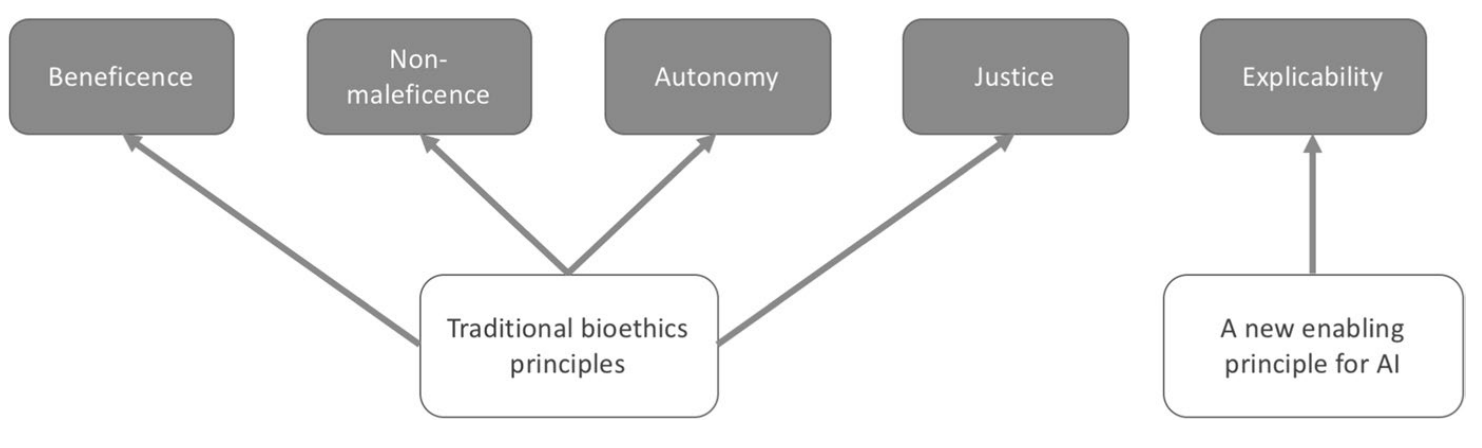
\includegraphics[width=0.75\linewidth]{Assets/AI Framework.png}
    \caption{An ethical framework for AI, formed of four traditional principles and a new one}
\end{figure}